%%%%%%%%%%%%%%%%%%%%%%%%%%%%%%%%%%%%%%%%%%%%%%%%%%%%%%%%%%%%%%%%%%%%%%%%%%%%%%%%
%%%% オペレーションズ・リサーチ　各種記事ひな形LaTeX2eファイル　2015-08-31版 %%%
%%%%%%%%%%%%%%%%%%%%%%%%%%%%%%%%%%%%%%%%%%%%%%%%%%%%%%%%%%%%%%%%%%%%%%%%%%%%%%%%
\documentclass[twocolumn, lastpage]{jarticle}

\overfullrule=5pt

\usepackage{amsmath,amssymb,amsfonts}
\usepackage{bm}
\usepackage{placeins}
\usepackage{graphicx}
\usepackage{subcaption}
\usepackage{nidanfloat}
\usepackage[numbers,sort]{natbib}
\usepackage{color}
\usepackage{url}
\usepackage{comment}

\usepackage{or}
\AtBeginDvi{\special{papersize=210mm,297mm}}

\vol{}
\vnum{}
\vyear{2026}

\jtitle{Gate Retrieval-Augmented Forecastingによる\\突発需要の予測}
\jauthor{奈良原　俊誠，斎藤　陽，橋本　朋樹，三川　健太}

\autfuri{ならはら　しゅんせい，さいとう　はる，はしもと　ともき}
\shozoku{東京都市大学メディア情報学部情報システム学科}
\shozoku{〒224--0015\enspace 神奈川県横浜市都筑区牛久保西3-3-1}

\autfuri{みかわ　けんた}
\shozoku{□□（株）☆☆☆☆部\\↑なんて書けばいいですかね汗}
\shozoku{〒000--0000\enspace ■■県★★市◆◆区▼▼▼▼0--0--0\\↑ここもです}

\begin{comment}
    
% 複数のメールアドレスは，見栄えに応じて改行を挿入すること
\shozoku{or-taro@sankaku.maru.ac.jp,\\ or-hanako@sankaku.maru.ac.jp}
% 住所のみ記載の例
\autfuri{おーあーる　じろう}
\shozoku{□□（株）☆☆☆☆部}
\shozoku{〒000--0000\enspace ■■県★★市◆◆区▼▼▼▼0--0--0}
% メールアドレスのみ記載の例
\autfuri{おーあーる　さぶろう}
\shozoku{◇◇大学▽▽学部}
\shozoku{or-saburo@shitasankaku.hishi.ac.jp}
% 外国所属で，住所のみ記載の例
\autfuri{ヤン　ヤンセン}
\shozoku{Department of AAA, BBB University of Technology}
\shozoku{P.O. Box 1111, 2222 GA Delft, The Netherlands}
% “論文・事例研究”・“論文・研究レポート”の場合，
% この位置に論文受付・採録に関係する日付が記載される
%\shozoku{受付 15.8.15　採択 15.8.15}
% “学生論文賞受賞論文”の場合↓
%\shozoku{
%○○大学大学院△△研究科 \\
%（現所属：□□（株）☆☆☆☆部） \\
%指導教員：尾有太郎　教授
%}
% “特集にあたって”の場合は，なし
\end{comment}


\begin{comment}
%% あらまし
% “特集記事”の場合に限り，必ず使用すること↓
\jabstract{
これは，オペレーションズ・リサーチ誌の各種記事の
ひな形（2015年8月31日版）である．
“特集記事”・“論文・事例研究”・“論文・研究レポート”
・“ORメモランダム”の場合に限り，サブタイトルを記載してもよい．
“特集記事”の場合に限り，あらましをここに，280字以内で記載し，
その下にキーワードを記載する．
}

\jkeywords{
特集記事キーワード1，キーワード2，
キーワードは三つ以上（指定のキーワードは特になし）
}
\end{comment}


\begin{document}
\special{papersize=210mm,297mm}
\normalsize
\setcounter{page}{1}
\setcounter{secondpage}{1}
\maketitle


%%%%%%%%%%%%%%%%%%%%%%%%%%%%%%%%%%%%%%%%%%%%%%%%%%%%%%%%%%%%%%%%%%%%%%%%%%%%%%%
\section{はじめに}
%%%%%%%%%%%%%%%%%%%%%%%%%%%%%%%%%%%%%%%%%%%%%%%%%%%%%%%%%%%%%%%%%%%%%%%%%%%%%%%
文字・活字文化の振興において，書籍や雑誌は基本的な文化資産であり，国家の文化水準を維持・向上させる上で極めて重要な役割を担っている．この役割を保障するための仕組みが再販売価格維持制度である~\cite{JBPA.2001}．同制度は出版社が定価を決定し，小売店に定価販売を義務付けるものであり，仮に価格競争が導入された場合に淘汰されうる多様な出版物を保護している．多様な出版物が保護された結果からなる多品種少量生産という特性に対応するため，出版業界では委託販売制度が広く採用されている~\cite{Shimomura.2005}．これは出版社が書店に販売を委託し，売れ残った場合に返本できる仕組みである．
しかしながら，需要に基づかない発注や配本が行われた場合，書店から出版社に対する過剰な返本が発生する．過剰な返本は物流網の圧迫や出版流通の観点から業界全体の深刻な課題となっている~\cite{Shuppan.2024}．そのため，返本率を低減し出版流通の効率化を図るためには，適切な需要予測が重要である．

書籍の需要予測は過去の販売冊数の推移を扱う時系列予測として位置づけられるが，本研究の対象である書籍のように多品種少量生産の特性を持つ時系列データの需要予測には，突発的な需要が予測で無視されやすいという点，データが限られた特定の系列の予測が困難であるという点の２つの課題がある．
前者は，全体の誤差を最小化するよう学習された一般的なモデルが，頻出するゼロ需要と少数の突出した需要を平均化してしまい，初版の発行や各種イベントに起因する急激な需要増加に対しても平坦な予測に陥りやすいという問題である．
後者は，新刊や販売実績の少ない書籍のようにデータ量が限られた系列において，モデルが需要の変動パターンを十分に学習できず，予測が困難になるという問題である．

これらの課題を解決する方法として，自然言語処理分野のRAG~\cite{Lewis.2020}を時系列予測へ拡張したRetrieval-Augmented Forecasting（RAF）が提案されている~\cite{Tire.2024}．RAFは，直近の需要変動に類似した過去のデータを検索・取得して予測に活用する仕組みにより，従来の単一系列モデルの限界を直接的に打破する強みを持つ．
1点目の問題である予測値の平坦化に対しては，過去のデータを直接参照することで突発的な需要スパイクのパターンを的確に捉えることを可能にする．さらに，2点目の問題である蓄積されたデータ量が乏しく需要の変動パターンを十分に学習できない場合でも，他系列の類似事例を横断的に参照することで予測を補完できる．
しかし，予測対象の入力系列であるローカルコンテキストに検索した参照ウィンドウをそのまま連結する従来のRAF，すなわちコンテキスト拡張型RAF~\cite{Tire.2024}には接合部の不連続性と無関係な参照ウィンドウの無条件混入という構造的問題がある．これらの問題は，参照ウィンドウを時間軸上でローカルコンテキストへ直接連結すること，および近傍探索が相対的な順位のみを返すために関連度の低い参照ウィンドウも一律に連結されることに起因する．

そこで本研究では，これらの2つの問題を構造的に解消するゲート付き融合型RAFであるGateRAFを提案する．
GateRAFは，ローカルコンテキストと各参照ウィンドウを同一のエンコーダで独立にエンコードするマルチストリームエンコードによって接合部の不連続性を根本的に排除し，ローカル要約ベクトルと各参照パッチとの関連度をスカラーゲートで評価するゲート機構によって無関係な参照の無条件混入を動的に抑制する．

提案手法の有効性を，経営科学系研究部会連合協議会が主催する令和7年度データ解析コンペティションより提供いただいた書籍POSデータを用いた実験により検証する．


%%%%%%%%%%%%%%%%%%%%%%%%%%%%%%%%%%%%%%%%%%%%%%%%%%%%%%%%%%%%%%%%%%%%%%%%%%%%%%%
\section{準備}
%%%%%%%%%%%%%%%%%%%%%%%%%%%%%%%%%%%%%%%%%%%%%%%%%%%%%%%%%%%%%%%%%%%%%%%%%%%%%%%
\subsection{問題設定}
本研究では，経営科学系研究部会連合協議会が主催する令和7年度データ解析コンペティションより提供いただいた書籍POSデータを使用する．本データは2024年の1年間にわたる全国35店舗分の書籍・雑誌の販売実績であり，約20万書名・約400万件の販売記録から構成される．各記録は販売日，店舗，書名，販売冊数等の情報を持つ．

本研究が目指すのは，書籍一点ごとに，将来その本が何冊売れるかを過去の販売実績から見積もることである．ただし，日々の販売冊数を平均的に当てること自体が目的ではない．書籍の売れ方には，刊行直後やメディア化・受賞などをきっかけとして短期間だけ販売が急増するスパイクと呼ばれる山が現れる．需要の大半は平常時のわずかな売上で占められる一方で，この山をいつ迎えるかは事前に読みにくい．山を見落とせば品切れによる販売機会の損失を招き，逆に過大に見積もれば過剰な発注と返本につながる．そこで本研究では，需要が跳ね上がる時期とその規模を的確に捉えつつ，平常時を誤って需要増と見なさないこと，すなわちスパイクの見落としと誤検知の双方を抑えることを中心的な課題とする．


\subsection{関連研究}
本研究の課題である突発的なスパイク需要の捕捉と少数系列からの学習に関連する既存研究を，時系列予測の基盤手法，間欠・突発需要予測，検索拡張型予測の3つの観点から整理する．

時系列予測の基盤手法としては，PatchTST~\cite{Nie.2023}等のTransformerベースの深層学習手法，確率的予測手法のDeepAR~\cite{Salinas.2020}やTFT~\cite{Lim.2021}，大規模事前学習基盤モデルChronos~\cite{Ansari.2024}が代表的手法として挙げられる．また間欠・突発需要予測は既に数多くの研究が存在しており，Croston法~\cite{Croston.1972}が基準手法として広く参照される．

RAG~\cite{Lewis.2020}を時系列予測へ拡張した検索拡張型予測(以下，RAF)は，予測対象のローカルコンテキストに類似した過去のウィンドウを検索データベースから取得し，それを予測に活用することで，単一系列モデルでは捕捉が困難な稀なスパイクパターンを系列横断的に参照できる．代表的な手法としてChronos~\cite{Ansari.2024}を基盤として検索した参照ウィンドウをローカルコンテキストへ時間軸方向に連結し，拡張した単一シーケンスとして一括エンコードするコンテキスト拡張型RAF(以下，ProtoRAF)が存在する\cite{Tire.2024}．ただしこの単純連結には接合部の不連続性と無関係な参照ウィンドウの混入という2つの構造的問題があり，TS-RAG~\cite{Ning.2025}およびTimeRAF~\cite{Zhang.2024}はそれぞれ潜在空間での融合やChannel Promptingによりこれを回避する．

ProtoRAFはこの参照を次のように取得する．まず，系列を長さ $L$ のウィンドウに区切って扱う．書名によって販売の規模は大きく異なるため，規模の違いに左右されず形の似た事例を集められるよう，各ウィンドウを標準化して形状をそろえたうえで比較する．予測対象のローカルコンテキストを $\bm{x} \in \mathbb{R}^{L}$ ，$\bm{x}$ を標準化したベクトルを $\tilde{\bm{x}} \in \mathbb{R}^{L} $ とおく．学習データから作った過去のウィンドウ集合 $\mathcal{D} = \{\bm{w}_i\}_{i=1}^{N}$ の各要素 $\bm{w}_i$ との距離 $d(\tilde{\bm{x}},\, \tilde{\bm{w}}_i)$ を測る．この距離が小さいほど形がよく似ており，最も似ている上位 $K$ 件を参照ウィンドウ $\bm{r}_k \in \mathbb{R}^{L}$（$k = 1, \dots, K$）として取得する：
    \begin{equation}
        \{\bm{r}_k\}_{k=1}^{K} = \underset{\bm{w}_i \in \mathcal{D}}{\operatorname{Top\text{-}K_{\mathrm{min}}}}\; d(\tilde{\bm{x}},\, \tilde{\bm{w}}_i)
    \end{equation}
ここで $\operatorname{Top\text{-}K_{\mathrm{min}}}$ は距離 $d$ が小さい順に $K$ 件を選ぶ操作であり，その計算には近傍検索~\cite{Johnson.2019}を用いる．未来の情報を使わないよう，$\mathcal{D}$ は予測時点より前のウィンドウのみで構成する．この検索は $\mathcal{D}$ の中で相対的に似ている $K$ 件を返すにすぎず，予測対象によく似た事例が存在しない場合でも常に $K$ 件が選び出される．

図~\ref{fig:protoraf}に示すように，ProtoRAFはこのローカルコンテキスト $\bm{x}$ の前方に参照ウィンドウ $\bm{r}_1, \dots, \bm{r}_K$ をそのまま連結し，拡張コンテキストを単一シーケンスとして一括エンコードする．パッチ数を $P$ ，エンコーダの埋め込み次元を $D$ とすると，以下のように表される：
    \begin{align}
        \bm{x}^{\mathrm{proto}} &= [\bm{r}_1 \,;\, \cdots \,;\,\bm{r}_K \,;\, \bm{x}] \\
        \bm{x}^{\mathrm{proto}} &\in \mathbb{R}^{(K+1)L} \\
        H^{\mathrm{proto}} &= \mathrm{Encode}(\bm{x}^{\mathrm{proto}}) \\
        H^{\mathrm{proto}} &\in \mathbb{R}^{(K+1)P \times D} \nonumber
    \end{align}
ここで角括弧内のセミコロンは，ベクトルやブロックを縦に並べて連結することを表す．$\bm{x}^{\mathrm{proto}}$ は参照ウィンドウをローカルコンテキストの前方に時間軸方向で連結した拡張コンテキストであり，$H^{\mathrm{proto}}$ はこれをエンコーダで符号化して得られるパッチ表現の系列である．
エンコーダが標準化~\cite{Kim.2022}に用いる平均と標準偏差 $(\mu, \sigma)$ は，ローカルコンテキストだけでなく参照ウィンドウまで連結した $\bm{x}^{\mathrm{proto}}$ 全体から計算される．
    \begin{figure*}[t]
        \centering
        
\includegraphics[width=0.75\linewidth]{figure/architecture/architecture_ProtoRAF.eps}
        \caption{ProtoRAFのアーキテクチャ概要}
        \label{fig:protoraf}
    \end{figure*}
    \begin{figure*}[t]
        \centering
        
\includegraphics[width=0.75\linewidth]{figure/architecture/architecture_GateRAF.eps}
        \caption{GateRAF（提案手法）のアーキテクチャ概要}
        \label{fig:gateraf}
    \end{figure*}

このProtoRAFには，参照ウィンドウとローカルコンテキストを1本の系列につなぐという構造そのものに起因して，接合部の不連続性と無関係な参照ウィンドウの混入という2つの問題が生じる．
前者は，連結した系列の継ぎ目をエンコーダが系列に実際に起きた値の変化と取り違えてしまう問題である．ProtoRAFは性質の異なる参照ウィンドウとローカルコンテキストを1本の長い系列としてつなぐため，その境目では値の水準や形が大きく食い違う．エンコーダはこの不自然な段差を，データに実際に起きた変化と区別できないまま学習してしまい，ローカルコンテキストの表現が歪んで予測精度が低下する．
また，この連結は標準化の基準もずらす．基盤モデルであるChronosは，入力系列を平均と標準偏差で標準化してから符号化する機構~\cite{Kim.2022}を備えている．ProtoRAFはこの入力に連結系列をそのまま渡すため，平均と標準偏差が，本来基準とすべきローカルコンテキストだけでなく参照ウィンドウまで連結した系列全体から計算され，ローカルコンテキストが本来のスケールから外れて処理される．

後者は，関連の薄い参照ウィンドウまでが予測にそのまま持ち込まれてしまう問題である．検索は予測対象とよく似た事例があるかどうかに関わらず，常に上位 $K$ 件を返す．そのため，似た事例が乏しい予測対象に対しても，関係の薄いウィンドウが参照ウィンドウとして連結されてしまう．ProtoRAFはこれらをローカルコンテキストと区別せずまとめてエンコードするため，無関係なウィンドウの情報まで取り込み，かえって予測精度が下がる．

提案手法は，これら2つの問題をマルチストリームエンコードとゲート機構によって構造的に解消する．


%%%%%%%%%%%%%%%%%%%%%%%%%%%%%%%%%%%%%%%%%%%%%%%%%%%%%%%%%%%%%%%%%%%%%%%%%%%%%%%
\section{提案手法}
%%%%%%%%%%%%%%%%%%%%%%%%%%%%%%%%%%%%%%%%%%%%%%%%%%%%%%%%%%%%%%%%%%%%%%%%%%%%%%%
\subsection{概要}
GateRAFは，ProtoRAFの2つの問題がいずれも，参照ウィンドウとローカルコンテキストを1本の系列につないでから一括で符号化することに由来する点に着目し，この符号化の流れ自体を見直すことで両者を解決する．基本となる考え方は，すべてをつなげてから処理するのではなく，ローカルコンテキストと各参照ウィンドウをそれぞれ別々に符号化し，最後に予測へ役立つ参照だけを選んで組み合わせることである．GateRAFの全体像を図~\ref{fig:gateraf}に示す．

GateRAFはこの考え方を2つの仕組みで実現する．1つ目はマルチストリームエンコードであり，ローカルコンテキストと各参照ウィンドウを同じエンコーダで別々に符号化する．つなぎ目をそもそも作らず，各ウィンドウを自身の値だけで標準化するため，継ぎ目をデータの変化と取り違える問題と，ローカルコンテキストが他のウィンドウに引きずられてスケールがずれる問題をまとめて解消する．2つ目はゲート機構であり，ローカルコンテキストとの関連の強さに応じて各参照に強弱をつける．関連の薄い参照の影響を小さく抑えることで，無関係なウィンドウが紛れ込む問題を防ぐ．


\subsection{マルチストリームエンコードとゲート付き融合}
GateRAFの予測は次の5つのステップからなり，その流れは図~\ref{fig:gateraf}に示す通りである．
    \begin{description}
        \item[ステップ1）] ローカルコンテキストのエンコード
        \item[ステップ2）] 参照ウィンドウの独立エンコード
        \item[ステップ3）] ローカル要約ベクトルの計算
        \item[ステップ4）] ゲートの計算
        \item[ステップ5）] ゲート付き融合
    \end{description}
ステップ1ではローカルコンテキストだけを符号化し，参照ウィンドウに影響されない標準化の基準を確保する．ステップ2では各参照ウィンドウを別々に符号化し，連結による接合部をそもそも作らない．ステップ3ではローカルコンテキストの表現を1本のベクトルにまとめ，参照の良し悪しを測る基準とする．ステップ4ではこの基準と各参照パッチを照らし合わせ，予測への役立ち度をゲートで見積もる．ステップ5ではゲートで重み付けした参照表現をローカルコンテキストの表現と統合し，予測に用いる．

    \paragraph{ステップ 1：ローカルコンテキストのエンコード}
    まず，予測対象のローカルコンテキスト $\bm{x}$ だけをエンコーダに入力し，そのパッチ表現 $H^{\mathrm{loc}}$ を得る：
        \begin{equation}
            H^{\mathrm{loc}} = \mathrm{Encode}(\bm{x}), \quad H^{\mathrm{loc}} \in \mathbb{R}^{P \times D}
        \end{equation}
    ここで $\mathrm{Encode}$ は基盤モデルのエンコーダであり，入力系列をその平均と標準偏差で標準化したうえでパッチ表現に変換する．この標準化に用いる平均と標準偏差を $(\mu, \sigma)$ と表す．ローカルコンテキスト $\bm{x}$ だけを入力するため，$(\mu, \sigma)$ は $\bm{x}$ 自身の平均と標準偏差として定まり，参照ウィンドウに含まれるスパイクに引きずられない．その結果，ローカルコンテキストは本来のスケールのまま処理され，連結系列から $(\mu, \sigma)$ を求めていたProtoRAFのようなスケールのずれが起こらない．

    \paragraph{ステップ 2：参照ウィンドウの独立エンコード}
    各参照ウィンドウ $\bm{r}_k$ をローカルコンテキストと同じエンコーダで個別に符号化し，参照ブロック $H^{\mathrm{ret}}_k$ を得る：
        \begin{align}
            H^{\mathrm{ret}}_k = \mathrm{Encode}(\bm{r}_k), \quad
            H^{\mathrm{ret}}_k \in \mathbb{R}^{P \times D} \\
            k = 1, \dots, K \nonumber
        \end{align}
    別々に符号化することで連結部分を作らず，接合部の不連続性が生じない．この段階では各参照を独立なブロック $H^{\mathrm{ret}}_k$ として保持し，ローカルコンテキストとも他の参照とも結合しない．

    \paragraph{ステップ 3：ローカル要約ベクトルの計算}
    $H^{\mathrm{loc}}$ をパッチ方向に平均プーリングし，ローカル要約ベクトル $\bar{\bm{h}}^{\mathrm{loc}}$ を得る：
        \begin{equation}
            \bar{\bm{h}}^{\mathrm{loc}} = \mathrm{Pool}(H^{\mathrm{loc}}), \quad \bar{\bm{h}}^{\mathrm{loc}} \in \mathbb{R}^{D}
        \end{equation}
    ここで $\mathrm{Pool}(\cdot)$ はパッチ方向の平均プーリングを表す．

    \paragraph{ステップ 4：ゲートの計算}
    このステップの目的は，各参照パッチを予測にどれだけ反映させるかを，ローカルコンテキストとの関連の強さに応じて決めることである．具体的には，ステップ3で得たローカル要約ベクトル $\bar{\bm{h}}^{\mathrm{loc}}$ と，各参照ブロックの第 $p$ パッチ $\bm{h}^{\mathrm{ret}}_{k,p} \in \mathbb{R}^{D}$ を，ゲートと呼ぶニューラルネットワークに入力し，両者の関連の強さを $0$ から $1$ の値 $g_{k,p}$ として出力する：
        \begin{align}
            g_{k,p} = \mathrm{GateMLP}(\bar{\bm{h}}^{\mathrm{loc}},\, \bm{h}^{\mathrm{ret}}_{k,p}), \quad
            g_{k,p} \in (0, 1) \\
            k = 1, \ldots, K,\ \ p = 1, \ldots, P \nonumber
        \end{align}
    $g_{k,p}$ は参照パッチの重みであり，$1$ に近いほどその参照を予測に強く反映し，$0$ に近いほど影響を抑える．関連の薄い参照を自動的に弱めることで，無関係なウィンドウの混入を防ぐのが狙いである．
    また，無関係な参照に最初から引きずられて学習が乱れないよう，ゲートは学習の初期にはほぼ閉じた状態，すなわち出力が $0$ に近い状態から始まるよう初期化する．これにより，モデルはまず信頼できるローカルコンテキストに基づいて予測を学習し，役立つ参照だけを学習の進行とともに徐々に取り込んでいく．


    \paragraph{ステップ 5：ゲート付き融合}
    最後に，ステップ4で求めた重みに従って各参照に強弱をつけ，ローカルコンテキストと一つにまとめる．まず，各参照ブロック $H^{\mathrm{ret}}_k$ の各パッチに，対応する重み $g_{k,p}$ を掛け，重み付き参照ブロック $\tilde{H}^{\mathrm{ret}}_k$ を得る．次に，ローカル表現と重み付けした全参照ブロックを結合して融合表現 $H^{\mathrm{gate}}$ とする：
        \begin{align}
            \tilde{H}^{\mathrm{ret}}_k &= \bm{g}_k \odot H^{\mathrm{ret}}_k, \quad \tilde{H}^{\mathrm{ret}}_k \in \mathbb{R}^{P \times D} \\
            & \hspace{25mm} k = 1, \ldots, K \nonumber \\
            H^{\mathrm{gate}} &= [H^{\mathrm{loc}} \,;\,
            \tilde{H}^{\mathrm{ret}}_1 \,;\, \cdots \,;\,
            \tilde{H}^{\mathrm{ret}}_K] \\
            H^{\mathrm{gate}} &\in \mathbb{R}^{(1+K)P \times D} \nonumber
        \end{align}

    ここで $\bm{g}_k = [g_{k,1}, \ldots, g_{k,P}]^\top$ は参照ブロック $k$ の各パッチのゲート値を並べたベクトルであり，$\odot$ は各パッチ $p$ の表現全体に同じ重み $g_{k,p}$ を掛ける演算を表す．関連の薄い参照ほど重みが小さくなるため，無関係なウィンドウの混入が抑えられる．参照表現とローカル表現を結合するのはこの最終段だけであり，それまでは互いに干渉しない．


\subsection{予測}
最後に，融合表現 $H^{\mathrm{gate}}$ から将来の販売冊数を予測する．$H^{\mathrm{gate}}$ には，ローカルコンテキストと，ゲートで重み付けした参照の情報がまとめられている．これを基盤モデルのデコーダに渡し，各分位点の予測を出力したうえで，符号化の際に施した標準化を元に戻す．分位点の集合を $Q$，予測する日数を $F$ とすると，以下のように表される：
    \begin{align}
        \hat{Y} &= \mathrm{RevNorm}(\mathrm{Decode}(H^{\mathrm{gate}}),\, \mu,\, \sigma) \\
        \hat{Y} &\in \mathbb{R}^{|Q| \times F} \nonumber
    \end{align}
問題設定で述べたとおり，予測は一つの値に絞らず，需要が取りうる範囲を複数の分位点として出力する．$\mathrm{RevNorm}: z \mapsto z\,\sigma + \mu$ は，ステップ1で得た平均と標準偏差 $(\mu, \sigma)$ を用いて，標準化されたスケールを実際の販売冊数のスケールへ戻す変換である．



%%%%%%%%%%%%%%%%%%%%%%%%%%%%%%%%%%%%%%%%%%%%%%%%%%%%%%%%%%%%%%%%%%%%%%%%%%%%%%%
\section{実験}
%%%%%%%%%%%%%%%%%%%%%%%%%%%%%%%%%%%%%%%%%%%%%%%%%%%%%%%%%%%%%%%%%%%%%%%%%%%%%%%
\subsection{概要}
提案手法が需要予測，とりわけ突発的なスパイク需要の捕捉に有効であるかを検証する．検証では次の2つの問いに答える．1つ目は，平常時のわずかな需要から突発的なスパイクまでを含めた予測全体の精度が，従来手法と比べて実際に向上するのかという問いである．2つ目は，GateRAFを支える2つの工夫，すなわち各ウィンドウを別々に符号化するマルチストリームエンコードと，関連の薄い参照を弱めるゲート機構が，それぞれ予測のどの側面を改善しているのかという問いである．

これらの問いに答えるため，時系列予測の基盤モデルに，提案手法の構成要素を一つずつ加えていく比較を行う．比較するのは，過去の類似事例を一切参照しない基盤モデルそのものであるBaseline，参照ウィンドウを入力系列にそのままつなぐ従来手法ProtoRAF，これにマルチストリームエンコードのみを加えたMulti-RAF，さらにゲート機構まで加えた提案手法GateRAFの4手法である．

評価は全体から個別へと掘り下げる．まず全系列を対象に全体的な精度を測る．このとき需要を一つの値で当てるのではなく，実際の需要が予測値を下回る確率をあらかじめ定めた水準に合わせた複数の予測値，すなわち分位点として評価する．たとえば確率0.9に対応する分位点は，実際の需要の9割が収まる高めの見積もりにあたる．こうして低め・中央・高めの見積もりを併せて評価することで，需要が上振れする可能性まで含めて精度を捉えられるためである．次に，改善が需要のどの局面で生じるかを見るため，実績値の大きさ別に誤差を分け，平常時を需要増と取り違える誤検知とスパイクの取りこぼしである見逃しの変化を調べる．さらに，予測の幅が実際の需要変動と対応しているかを確認し，どの時点で需要増に備えるべきかという実務的な示唆につながるかを検討する．最後に，全体の平均には現れない個々の挙動を確かめるため，スパイクの現れ方が異なる代表的な系列で，予測が実際のスパイクに追従できているかを可視化する．


\subsection{データ整形}
本研究では書名ごとの需要推移を予測対象とするため，まず店舗間の差異を捨象し，同一の書名・日付に対する販売冊数を全店舗にわたって合算することでPOS販売冊数の時系列を構築した．その上で，予測対象として適した系列を得るために以下の前処理を施した．第一に，年間総販売冊数が366冊，すなわち一日あたり平均1冊に満たない書籍は販売実績が著しく予測に必要な情報量を欠くため除外した．第二に，巻数違い等の同一作品を作品シリーズ単位へ統合し，一つの需要系列として扱った．巻数の違いは販売管理上の区別にすぎず，需要の対象としては同一の作品とみなすべきと考えたためだ．第三に，販売記録の存在しない日を欠測ではなくゼロ需要とみなして補完し，全書名と全日付を網羅する完全パネルデータを構築した．以上の処理により，最終的に約40万件のデータを得た．

得られたデータでは，POS販売冊数の平均が約3.68冊，標準偏差13.65冊と平均に対して分散が大きく，さらにゼロ販売日の割合が42.9\%に達する．このことは，平常時の間欠的なゼロ需要と突発的なスパイク需要が混在するという，本研究が対象とする需要構造を端的に表している．


\subsection{実験条件}
全手法は，膨大な時系列データであらかじめ学習された予測モデル，すなわち時系列予測の基盤モデルであるChronos~\cite{Ansari.2024}を土台とする．具体的には，その軽量かつ高速版であるChronosBoltを用い，モデル全体を学習し直すのではなく，ごく少数の追加パラメータのみを調整して本データに適応させるDoRA~\cite{Liu.2024}によってファインチューニングした．追加パラメータの規模は，その代表的手法であるLoRA~\cite{Hu.2022}のランクで $r=8$ とした．

予測の単位は，書名ごとの需要系列である．各系列から直近 $L=128$ 日分を切り出してローカルコンテキストとし，これをもとに続く $F=64$ 日分の販売冊数を予測する．予測値は一つの値ではなく，3つの分位点 $\tau \in \{0.1,\, 0.5,\, 0.9\}$ として出力する．ここで分位点 $\tau$ とは，実際の需要が予測値を下回る確率が $\tau$ となる水準である．学習には，これら3つの分位点を同時に当てに行うピンボール損失~\cite{Koenker.1978}を用いる．参照ウィンドウは，1回の予測につきローカルコンテキストに形の似た上位 $K=3$ 件を検索して用いる．

比較するのはBaseline，ProtoRAF，Multi-RAF，GateRAFの4手法である．このうち，ProtoRAFとMulti-RAFの比較はマルチストリームエンコードの寄与を，Multi-RAFとGateRAFの比較はゲート機構の効果を，それぞれ切り分けて確かめる役割をもつ．

\subsection{実験結果}
\subsubsection{予測精度の算出}
表~\ref{tab:metric_comparison} に，全系列と全予測期間で算出した平均絶対誤差（以下，MAE）と二乗平均平方根誤差（以下，RMSE）を分位点ごとに示す．いずれも値が小さいほど予測が実績に近い．全体として，提案手法GateRAFは多くの指標で最も誤差が小さく，とくに中央（$\tau=0.5$）と上側（$\tau=0.9$）で従来手法を上回った．以下，Baselineに構成要素を一つずつ加え，各要素の寄与を順にみる．

参照を入力にそのままつなぐProtoRAFは，Baselineとほぼ同じ誤差にとどまった（$\tau=0.5$のMAEはともに $3.05$，$\tau=0.9$のRMSEはともに $27.0$ 程度）．参照を単純につなぐだけでは改善につながっていない．

マルチストリームエンコードを加えたMulti-RAFでは誤差が大きく下がり，$\tau=0.9$のMAEは $6.85$ から $4.97$ へ，RMSEは $27.02$ から $13.36$ へ改善した．これは標準化の基準のずれが解消されたためと考えられる．ProtoRAFは標準化の平均と標準偏差を参照ウィンドウまで含めて計算するため，大きなスパイクを含む参照が混じるとローカルコンテキストが過大なスケールで標準化され，上側分位点が上振れしていたとみられる．Multi-RAFはローカルコンテキストを単独で標準化するため，このずれが生じにくい．ただし下側（$\tau=0.1$）のMAEは $3.66$ から $3.78$ へわずかに悪化しており，効果は中央から上側に偏っている．

さらにゲート機構を加えたGateRAFでは，低い分位点を中心に誤差が下がり，$\tau=0.1$のMAEは $3.78$ から $3.63$ へ，$\tau=0.5$は $2.81$ から $2.75$ へ改善した．一方 $\tau=0.9$のMAEは $4.97$ から $5.01$ とほぼ同水準であり，ゲート機構による改善は低い分位点（$\tau=0.1$），すなわち平常時の小さな需要の予測に主に現れている．
    \begin{table*}[t]
        \caption{各モデルおよび分位点レベルにおける MAE および RMSE の比較}
        \label{tab:metric_comparison}
        \centering
        \begin{tabular}{lrrrrrr}
            \hline
            & \multicolumn{6}{c}{分位点} \\
            \cline{2-3} \cline{4-5} \cline{6-7}
            \multicolumn{1}{c}{モデル} & \multicolumn{2}{c}{$\tau=0.1$} & \multicolumn{2}{c}{$\tau=0.5$} & \multicolumn{2}{c}{$\tau=0.9$} \\
            \cline{2-3} \cline{4-5} \cline{6-7}
            & \multicolumn{1}{c}{MAE} & \multicolumn{1}{c}{RMSE} & \multicolumn{1}{c}{MAE} & \multicolumn{1}{c}{RMSE} & \multicolumn{1}{c}{MAE} & \multicolumn{1}{c}{RMSE} \\
            \hline\hline
            \textbf{GateRAF} & \textbf{3.6339} & \textbf{13.5293} & \textbf{2.7452} & \textbf{12.2025} & 5.0136 & \textbf{13.3030} \\
            \textbf{Multi-RAF} & 3.7766 & 13.6118 & 2.8117 & 12.2594 & \textbf{4.9745} & 13.3570 \\
            \textbf{ProtoRAF} & 3.6604 & 13.7593 & 3.0467 & 12.9622 & 6.8549 & 27.0196 \\
            \textbf{Baseline} & 3.6501 & 13.7476 & 3.0460 & 12.9603 & 6.8512 & 27.0050 \\
            \hline
        \end{tabular}
    \end{table*}


\subsubsection{スパイク強度別の予測精度}
需要が平常時にあるのか急増しているのかによって予測の難しさは大きく異なる．そこで各時点の実績値を，その系列自身の平均からどれだけ離れているかを標準偏差を単位として測った系列内 $z$ スコアに変換し，この値の大きさごとに予測誤差を比べた．$z$ スコアが大きい時点ほど需要が平常を大きく上回るスパイクであり，逆に小さい時点ほど需要が平常を下回る穏やかな状態にあたる．表~\ref{tab:mae_rmse_vs_zscore}に，$z$ スコアの帯ごとのMAEとRMSEを示す．

まず，$z$ スコアが $-1$ を下回る，需要が平常を大きく下回る穏やかな時点に着目する．以下ではこの帯を静穏域と呼ぶ．表~\ref{tab:mae_rmse_vs_zscore}が示すように，$\tau=0.5$ のMAEはBaselineの $2.66$ に対しGateRAFは $1.84$ と全モデル中で最も小さく，平常時を過大に見積もる誤りが抑えられている．この帯では従来手法の過大予測がとくに目立ち，$\tau=0.9$ のRMSEはGateRAFが $9.70$ であるのに対し，ProtoRAFは $29.11$ と大幅に大きい．標準化の基準のずれが，スパイクのない穏やかな需要帯においても過大な予測を招いていたことがうかがえる．

ゲート機構の寄与も，この静穏域の低い分位点に現れる．$\tau=0.1$ の静穏域におけるMAEは，Multi-RAFの $1.03$ に対しGateRAFは $0.85$ へと下がった．関連の薄い参照を弱めることで，平常時に無関係なスパイク事例へ引っ張られる過剰な反応が抑えられたためと考えられる．一方で，改善は穏やかな時点に限られない．$z$ スコアが $2$ を上回る，需要が大きく跳ね上がる時点でも，$\tau=0.5$ のMAEはGateRAFが全モデル中で最良である．$z$ スコアが $2$ から $3$ の帯ではBaselineの $12.41$ から $11.28$ へ，$3$ を超える帯では $26.25$ から $24.76$ へと誤差が下がっている．以上から，提案手法は平常時の過大な予測を抑えつつ，突発的なスパイクの捕捉も両立できていると考えられる．
    \begin{table*}[t]
        \caption{系列内$z$スコアビン別のMAEおよびRMSE}
        \label{tab:mae_rmse_vs_zscore}
        \centering
        \resizebox{\textwidth}{!}{
        \begin{tabular}{lrrrrrrrrrrrrrrrr}
            \hline
            & \multicolumn{2}{c}{$<$-1} & \multicolumn{2}{c}{-1--0} & \multicolumn{2}{c}{0--0.5} & \multicolumn{2}{c}{0.5--1} & \multicolumn{2}{c}{1--1.5} & \multicolumn{2}{c}{1.5--2} & \multicolumn{2}{c}{2--3} & \multicolumn{2}{c}{$>$3} \\
            \cline{2-17}
            \multicolumn{1}{c}{モデル} & MAE & RMSE & MAE & RMSE & MAE & RMSE & MAE & RMSE & MAE & RMSE & MAE & RMSE & MAE & RMSE & MAE & RMSE \\
            \hline\hline
            \multicolumn{17}{l}{$\tau=0.1$} \\
            \quad \textbf{GateRAF} & \textbf{0.85} & \textbf{2.88} & 1.57 & 4.57 & \textbf{4.65} & \textbf{9.48} & \textbf{5.98} & \textbf{11.86} & \textbf{7.18} & \textbf{15.81} & \textbf{8.42} & \textbf{17.66} & \textbf{14.72} & \textbf{39.32} & \textbf{28.08} & 63.94 \\
            \quad \textbf{Multi-RAF} & 1.03 & 3.01 & 1.71 & 4.67 & 4.77 & 9.56 & 6.15 & 12.00 & 7.36 & 15.92 & 8.59 & 17.80 & 14.84 & 39.68 & 28.24 & \textbf{63.94} \\
            \quad \textbf{ProtoRAF} & 0.89 & 3.09 & 1.47 & 4.39 & 4.77 & 9.79 & 6.20 & 12.22 & 7.51 & 16.47 & 8.79 & 18.36 & 15.45 & 40.54 & 28.58 & 64.37 \\
            \quad \textbf{Baseline} & 0.89 & 3.08 & \textbf{1.46} & \textbf{4.38} & 4.76 & 9.77 & 6.19 & 12.21 & 7.50 & 16.45 & 8.78 & 18.35 & 15.44 & 40.51 & 28.56 & 64.35 \\
            \hline
            \multicolumn{17}{l}{$\tau=0.5$} \\
            \quad \textbf{GateRAF} & \textbf{1.84} & \textbf{3.15} & \textbf{1.21} & 3.78 & \textbf{2.96} & 7.32 & \textbf{3.92} & \textbf{9.90} & \textbf{4.94} & \textbf{13.12} & \textbf{6.05} & \textbf{14.98} & \textbf{11.28} & \textbf{35.30} & \textbf{24.76} & 61.12 \\
            \quad \textbf{Multi-RAF} & 1.94 & 3.23 & 1.26 & \textbf{3.77} & 3.01 & \textbf{7.29} & 4.03 & 9.95 & 5.07 & 13.14 & 6.19 & 15.17 & 11.47 & 35.98 & 24.84 & \textbf{61.00} \\
            \quad \textbf{ProtoRAF} & 2.66 & 6.21 & 1.40 & 5.13 & 3.14 & 8.22 & 4.22 & 10.73 & 5.39 & 13.82 & 6.50 & 15.74 & 12.42 & 36.57 & 26.26 & 62.31 \\
            \quad \textbf{Baseline} & 2.66 & 6.21 & 1.40 & 5.14 & 3.13 & 8.22 & 4.22 & 10.73 & 5.39 & 13.82 & 6.50 & 15.75 & 12.41 & 36.55 & 26.25 & 62.29 \\
            \hline
            \multicolumn{17}{l}{$\tau=0.9$} \\
            \quad \textbf{GateRAF} & \textbf{6.19} & 9.70 & 4.52 & 9.50 & 4.47 & 8.98 & 4.74 & \textbf{10.04} & 4.56 & \textbf{10.64} & 4.89 & \textbf{12.42} & \textbf{8.39} & \textbf{30.16} & 18.81 & 55.93 \\
            \quad \textbf{Multi-RAF} & 6.27 & \textbf{9.64} & \textbf{4.46} & \textbf{9.43} & \textbf{4.41} & \textbf{8.92} & \textbf{4.73} & 10.18 & \textbf{4.51} & 10.65 & \textbf{4.88} & 12.59 & 8.57 & 31.39 & \textbf{18.73} & \textbf{55.86} \\
            \quad \textbf{ProtoRAF} & 9.48 & 29.11 & 6.57 & 27.12 & 6.33 & 24.03 & 5.75 & 25.13 & 4.79 & 11.83 & 5.39 & 15.07 & 9.56 & 33.12 & 20.74 & 58.00 \\
            \quad \textbf{Baseline} & 9.49 & 29.17 & 6.56 & 27.09 & 6.33 & 24.02 & 5.75 & 25.16 & 4.80 & 11.83 & 5.39 & 15.08 & 9.56 & 33.15 & 20.72 & 57.99 \\
            \hline
        \end{tabular}}
    \end{table*}


\subsubsection{時間近接性}
予測の誤りが実際のスパイクからどれだけ離れた時点で生じているかを調べる．分析の条件は次のとおりである．スパイクは系列内 $z$ スコアが $2.0$ 以上となる時点と定める．$\tau=0.5$ の予測を対象とし，モデルが誤った各時点について，最も近い実際のスパイクまでの日数 $\Delta$ を，そのスパイクより前か後かを符号として測る．スパイクがない時点を誤ってスパイクと予測する誤検知をFalse Positive（以下，FP），実際のスパイクを予測できない見逃しをFalse Negative（以下，FN）と呼び，FPにおける $\Delta$ の分布を図~\ref{Fig:temporal_proximity_fp}に，FNにおける $\Delta$ の分布を図~\ref{Fig:temporal_proximity_fn}に示す．いずれの図でも，最も外側のビンは付近10日以内に対応するスパイクが存在しないことを表す．

FPのうち，近くに実際のスパイクが見当たらないノイズ的な誤り，すなわち $|\Delta| \geq 10$ のものの割合は，ProtoRAFの $59.1\%$ に対しGateRAFは $49.6\%$ と低い．つまりGateRAFの誤検知の多くは，実際のスパイクに近接したタイミングのずれによるものである．FNでも同様に，GateRAFはスパイク付近で予測を上方修正する挙動を示す．これは，ゲート機構がローカル文脈に類似した参照パッチのみを選んで通すことで，無関係な参照の混入を時間軸の上でも抑えているためと考えられる．
    \begin{figure}
        \centering
        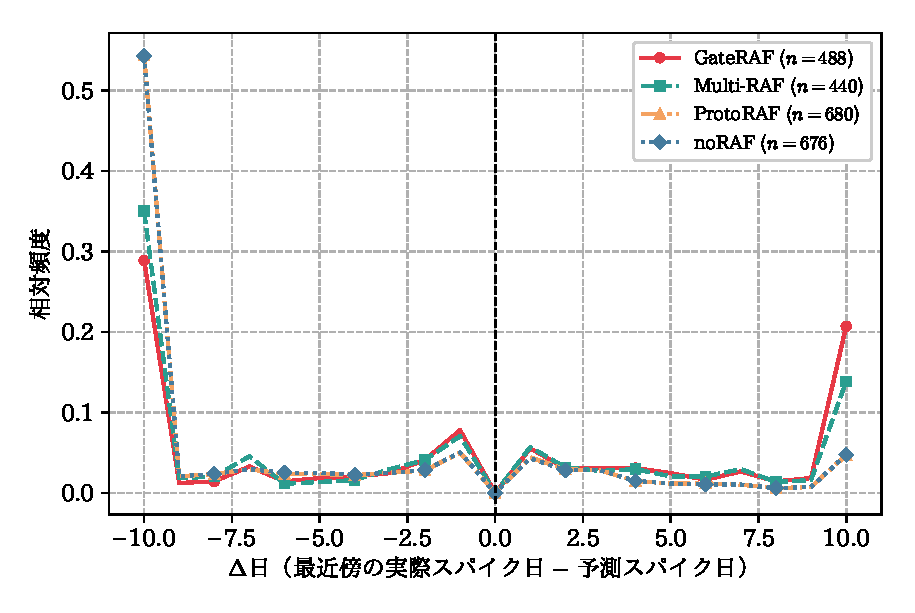
\includegraphics[width=\linewidth]{figure/temporal_proximity/temporal_proximity_fp_q0.5.eps}
        \caption{誤検知FPの $\Delta$日分布}
        \label{Fig:temporal_proximity_fp}
    \end{figure}
    \begin{figure}
        \centering
        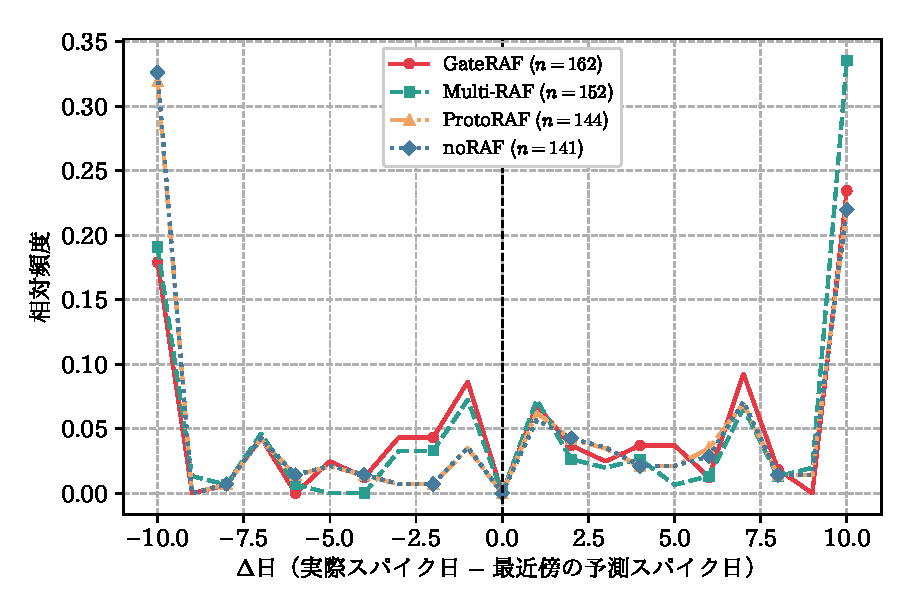
\includegraphics[width=\linewidth]{figure/temporal_proximity/temporal_proximity_fn_q0.5.eps}
        \caption{見逃しFNの $\Delta$日分布}
        \label{Fig:temporal_proximity_fn}
    \end{figure}


\subsubsection{予測区間幅の比較}
モデルは予測値を分位点として出力するため，高い分位点 $\tau=0.9$ と低い分位点 $\tau=0.1$ の予測値の差を，その時点で見込んだ需要のばらつきの幅，すなわち予測区間の幅とみなせる．この幅が広いほど，モデルはその時点の需要を読みにくいと判断していることになる．ここでは，この予測区間の幅が，実際に需要が跳ね上がる時点とどれだけ対応しているかを調べる．具体的には，全時点を予測区間の幅の順に並べて同数ずつ10個のグループに分け，グループごとに実績の系列内 $z$ スコアの平均を求める．予測区間が広いグループほど実際の $z$ スコアも大きい，すなわち右上がりの関係になっていれば，モデルは需要が急増する時点でこそ区間を広げており，不確実性を実際の需要変動に合わせられていることになる．

図~\ref{Fig:interval_calibration}より，GateRAFとMulti-RAFでは予測区間の幅が広がるにつれて $z$ スコアの平均が $-0.34$ から $+0.32$ へと一貫して上昇しており，広い予測区間が実際のスパイク発生時点に集中していることがわかる．一方，ProtoRAFでは $-0.06$ から $+0.14$ までとほとんど変化せず，予測区間の幅が実需の変動とほとんど連動していない．GateRAFとMulti-RAFでこの傾向がほぼ一致することから，この連動は主にマルチストリームエンコードによるスケールの安定化によって生じていると考えられる．

この結果は，予測区間の幅が単なる出力のばらつきではなく，需要が変動しやすい時点を事前に示す手がかりとして機能していることを示唆する．点予測ではスパイクの正確な時刻や大きさまで言い当てることは難しいが，予測区間が実需の変動と連動していれば，一点を当てられなくとも「この時点は需要が跳ねうる」という不確実性そのものを表現できる．まれで予測の難しいスパイクを対象とする本研究では，一点を当てにいく点予測に加えて，不確実性を幅として表現できることにも独自の意義があると考えられる．また，この連動が主にマルチストリームエンコードに由来することは，標準化の基準を正したことが，連結による歪みで頭打ちになっていた上側分位点を，実際の需要変動に応答できる状態へ回復させたためと解釈できる．逆にProtoRAFのように区間幅が実需と無関係であれば，区間の広さは需要の変動について何も語らず，不確実性の出力は意思決定の手がかりにならない．以上より，提案手法は需要に備えるべき時点を予測区間という形で時点ごとに示せると考えられ，スパイクの見落としと誤検知の双方を抑えるという本研究の課題に対し，点予測の精度向上とは別の側面から寄与しうる．
    \begin{figure}
        \centering
        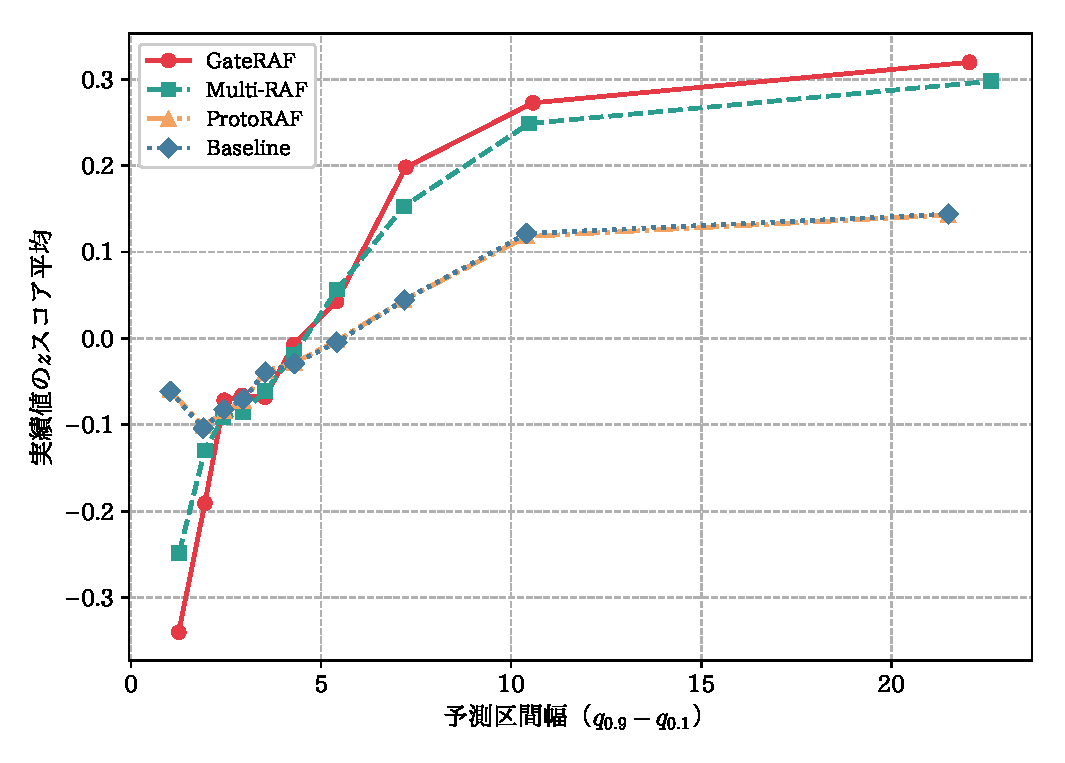
\includegraphics[width=\linewidth]{figure/interval_calibration.eps}
        \caption{予測区間の幅ごとの実績 $z$ スコア平均}
        \label{Fig:interval_calibration}
    \end{figure}


\subsubsection{書名別事例分析}
これまでの全体指標は平均的な精度の改善を表すが，各モデルが個々のスパイクにどう反応するかまでは見えない．そこで，スパイクの現れ方が異なる代表的な2つの系列を取り上げ，$\tau=0.5$ の予測値の時系列を実績と重ねて比較する．その様子を図~\ref{fig:book_examples}に示す．図中では，黒の実線が実績を表し，赤の実線がGateRAF，青の破線がMulti-RAF，緑の点線がProtoRAF，橙の一点鎖線がBaselineの予測を表す．これにより，マルチストリームエンコードとゲート機構がスパイクへの追従にどう寄与するかを具体的に確かめる．

    \paragraph{書籍A}
    この系列は，予測期間の冒頭で実績が急増し，系列内 $z$ スコアが最大 $3.6$ に達したのち，急速に減衰するパターンを示す．図~\ref{fig:book_bocchi}を見ると，GateRAFはこの減衰にほぼ沿って予測を下げ，MAEは $2.39$ にとどまった．一方ProtoRAFとBaselineは，実績が下がっても高い予測を維持し続け，MAEは $7.81$ と大きい．これは，ProtoRAFが連結系列全体から標準化の基準を取るために予測のスケールが高止まりし，需要が落ち着いたあとも過大な予測から抜け出せないことを表していると考えられる．標準化の基準をローカルコンテキストだけから取るGateRAFは，この高止まりを避けられている．

    \paragraph{書籍B}
    この系列は，予測期間の中盤にあたる20日目前後で実績が急増し，系列内 $z$ スコアが最大 $5.8$ に達するパターンを示す．図~\ref{fig:book_crossword}より，GateRAFとMulti-RAFはこの急増に合わせて予測を立ち上げており，MAEはそれぞれ $1.59$，$1.88$ である．対してProtoRAFとBaselineは予測値がほぼゼロのまま動かず，スパイクをまったく捉えられなかった．ProtoRAFのMAEは $2.96$ である．Multi-RAFの段階ですでに検出できていることから，このスパイクの予兆は，参照ウィンドウを個別に符号化して取り込むマルチストリームエンコードによって引き出されていると解釈できる．参照を持たないBaselineはもとより，参照を単純に連結するだけのProtoRAFでも，取得した類似事例のスパイクが予測に現れていない．
        \begin{figure*}[tb]
            \centering
            \begin{subfigure}[t]{0.8\textwidth}
                \centering
                
\includegraphics[width=\linewidth]{figure/figure_book/figure_book_bocchi.eps}
                \caption{書籍A}
                \label{fig:book_bocchi}
            \end{subfigure}
            \vspace{1em}
            \begin{subfigure}[t]{0.8\textwidth}
                \centering
                
\includegraphics[width=\linewidth]{figure/figure_book/figure_book_crossword.eps}
                \caption{書籍B}
                \label{fig:book_crossword}
            \end{subfigure}
            \caption{各系列における予測と実績の比較}
            \label{fig:book_examples}
        \end{figure*}

以上の2例は，いずれもマルチストリームエンコードの働きを端的に表している．すなわち，標準化の基準をローカルコンテキストに限ることで過大な予測の高止まりを防ぎ，参照ウィンドウを個別に取り込むことで他系列のスパイクを予測に反映させる，という2つの働きである．これらの例でGateRAFとMulti-RAFの挙動がほぼ重なることは，スパイクへの追従そのものが主にマルチストリームエンコードによって実現されていることを裏づけており，ゲート機構の寄与は，全体指標で見たとおり平常時の予測の調整という別の側面に現れると考えられる．


%%%%%%%%%%%%%%%%%%%%%%%%%%%%%%%%%%%%%%%%%%%%%%%%%%%%%%%%%%%%%%%%%%%%%%%%%%%%%%%
\section{おわりに}
%%%%%%%%%%%%%%%%%%%%%%%%%%%%%%%%%%%%%%%%%%%%%%%%%%%%%%%%%%%%%%%%%%%%%%%%%%%%%%%
本研究では，多品種少量生産という特性を持つ出版販売データに対する需要予測，特に突発的なスパイク需要の捕捉を目的として，ゲート付き融合型RAFであるGateRAFを提案した．GateRAFは，既存のコンテキスト拡張型RAFが抱える2つの構造的問題，すなわち参照ウィンドウの連結に起因する時系列の接合部不連続性と，無関係な参照系列の無条件混入を，マルチストリームエンコードとゲート機構という独立した設計上の工夫によってそれぞれ解消する．

数値実験の結果，GateRAFは予測全体の精度において，従来手法であるProtoRAFと，過去の事例を参照しないBaselineの双方を上回ることが確認された．
また，マルチストリームエンコードとゲート機構が予測の異なる側面を改善していることが明らかになった．
\begin{comment}
前者は，事例ごとに値の大きさをそろえる基準がずれる問題を根本から正すことで，平常時のわずかな需要から急に跳ね上がったスパイクまで，さまざまな大きさの需要に対する予測を安定させる役割を主に担う．後者は，平常時を誤って需要の増加と見なす誤りを減らし，スパイクを捉える時期のずれを小さくすることで，前者の効果を補う．
\end{comment}

今後の課題は3点である．第一に，参照ウィンドウの検索が波形の形状の類似のみに基づく点である．需要が動く背景は形状だけでは捉えきれないこともあり，形状以外の観点から似た事例を選ぶ類似尺度を検討したい．第二に，参照の統合がそれぞれの強弱づけにとどまる点である．本研究のゲート機構は各参照に強弱をつけて取捨選択するにとどまり，参照を組み合わせた新たな表現を作るには至っていない．取捨選択にとどまらない統合の仕組みを取り入れれば，さらなる精度向上が期待できる．第三に，ゲート機構の調整に学習を要する点である．本研究ではゲート機構を学習によって調整したが，計算コストを抑える観点からは，追加学習を行わずに参照を活用するゼロショットでの利用も有望である．

%% 謝辞
\shaji
---

%%%%%%%% 参考文献 %%%%%%%%%%%%%%%%%%%%%%%%%%%%%%%%%%%%%%%%%%%%%%%%%%%%%%%%%%%%%%
\begin{thebibliography}{99}

\bibitem[日本書籍出版協会(2001)]{JBPA.2001}
日本書籍出版協会,
「再販制度」,
\url{https://www.jbpa.or.jp/resale/}, 2001.

\bibitem[下村(2005)]{Shimomura.2005}
下村昭夫,
``日本における出版産業の現状と課題'',
\textit{出版研究}, vol.~35, pp.~95--102, 2005.

\bibitem[全国出版協会・出版科学研究所(2024)]{Shuppan.2024}
全国出版協会・出版科学研究所,
『出版指標年報 2024年版』,
全国出版協会, 2024.

\bibitem[Lewis~et~al.(2020)]{Lewis.2020}
P.~Lewis, E.~Perez, A.~Piktus, F.~Petroni, V.~Karpukhin, N.~Goyal, H.~K\"{u}ttler, M.~Lewis, W.-T.~Yih, T.~Rockt\"{a}schel, S.~Riedel and D.~Kiela,
``Retrieval-Augmented Generation for Knowledge-Intensive {NLP} Tasks,''
in \textit{Advances in Neural Information Processing Systems}, vol.~33, pp.~9459--9474, 2020.

\bibitem[Tire~et~al.(2024)]{Tire.2024}
K.~Tire, E.~O.~Taga, M.~E.~Ildiz and S.~Oymak,
``Retrieval Augmented Time Series Forecasting,''
arXiv:2411.08249, 2024.

\bibitem[Nie~et~al.(2023)]{Nie.2023}
Y.~Nie, N.~H.~Nguyen, P.~Sinthong and J.~Kalagnanam,
``A Time Series is Worth 64 Words: Long-term Forecasting with Transformers,''
in \textit{Proceedings of the International Conference on Learning Representations}, 2023.

\bibitem[Salinas~et~al.(2020)]{Salinas.2020}
D.~Salinas, V.~Flunkert, J.~Gasthaus and T.~Januschowski,
``{DeepAR}: Probabilistic Forecasting with Autoregressive Recurrent Networks,''
\textit{International Journal of Forecasting}, vol.~36, no.~3, pp.~1181--1191, 2020.

\bibitem[Lim~et~al.(2021)]{Lim.2021}
B.~Lim, S.~\"{O}.~Ar{\i}k, N.~Loeff and T.~Pfister,
``Temporal Fusion Transformers for Interpretable Multi-Horizon Time Series Forecasting,''
\textit{International Journal of Forecasting}, vol.~37, no.~4, pp.~1748--1764, 2021.

\bibitem[Ansari~et~al.(2024)]{Ansari.2024}
A.~F.~Ansari, L.~Stella, C.~Turkmen, X.~Zhang, P.~Mercado, H.~Shen, O.~Shchur,
S.~S.~Rangapuram, S.~P.~Arango, S.~Kapoor, J.~Zschiegner, D.~C.~Maddix,
H.~Wang, M.~W.~Mahoney, K.~Torkkola, A.~G.~Wilson, M.~Bohlke-Schneider and Y.~Wang,
``Chronos: Learning the Language of Time Series,''
arXiv:2403.07815, 2024.

\bibitem[Croston(1972)]{Croston.1972}
J.~D.~Croston,
``Forecasting and Stock Control for Intermittent Demands,''
\textit{Operational Research Quarterly}, vol.~23, no.~3, pp.~289--303, 1972.

\bibitem[Ning~et~al.(2025)]{Ning.2025}
K.~Ning, Z.~Pan, Y.~Liu, Y.~Jiang, J.~Y.~Zhang, K.~Rasul, A.~Schneider, L.~Ma, Y.~Nevmyvaka and D.~Song,
``TS-RAG: Retrieval-Augmented Generation based Time Series Foundation Models are Stronger Zero-Shot Forecaster,''
arXiv:2503.07649, 2025.

\bibitem[Zhang~et~al.(2024)]{Zhang.2024}
H.~Zhang, C.~Xu, Y.-F.~Zhang, Z.~Zhang, L.~Wang, J.~Bian and T.~Tan,
``{TimeRAF}: Retrieval-Augmented Foundation Model for Zero-Shot Time Series Forecasting,''
arXiv:2412.20810, 2024.

\bibitem[Johnson~et~al.(2019)]{Johnson.2019}
J.~Johnson, M.~Douze and H.~J\'{e}gou,
``Billion-Scale Similarity Search with {GPU}s,''
\textit{IEEE Transactions on Big Data}, vol.~7, no.~3, pp.~535--547, 2019.

\bibitem[Kim~et~al.(2022)]{Kim.2022}
T.~Kim, J.~Kim, Y.~Tae, C.~Park, J.-H.~Choi and J.~Choo,
``Reversible Instance Normalization for Accurate Time-Series Forecasting against Distribution Shift,''
in \textit{Proceedings of the International Conference on Learning Representations}, 2022.

\bibitem[Liu~et~al.(2024)]{Liu.2024}
S.-Y.~Liu, C.-Y.~Wang, H.~Yin, P.~Molchanov, Y.-C.~F.~Wang, K.-T.~Cheng and M.-H.~Chen,
``{DoRA}: Weight-Decomposed Low-Rank Adaptation,''
in \textit{Proceedings of the International Conference on Machine Learning}, 2024.

\bibitem[Hu~et~al.(2022)]{Hu.2022}
E.~J.~Hu, Y.~Shen, P.~Wallis, Z.~Allen-Zhu, Y.~Li, S.~Wang, L.~Wang and W.~Chen,
``{LoRA}: Low-Rank Adaptation of Large Language Models,''
in \textit{Proceedings of the International Conference on Learning Representations}, 2022.

\bibitem[Koenker~\&~Bassett(1978)]{Koenker.1978}
R.~Koenker and G.~W.~Bassett,
``Regression Quantiles,''
\textit{Econometrica}, vol.~46, no.~1, pp.~33--50, 1978.

\end{thebibliography}

\end{document}
